\documentstyle[11pt, titlepage, ps, epsf]{article}
\setlength{\topmargin}{0.1in}
\setlength{\oddsidemargin}{-0.1in}
\setlength{\textheight}{9.3in}
\setlength{\textwidth}{6.5in}
\addtolength{\topmargin}{-0.5in}
\setlength{\footskip}{1in}
\setlength{\footheight}{0.5in}
\setlength{\parindent}{0in}		% no paragraph indent
\setlength{\parskip}{2ex}		% space between paragraphs

\def\not{\mbox{${\tt '\backslash+'/1}$}}

\newcommand{\version}{Version 1.4.1}

\newcommand{\demo}[1]{\hspace*{1.5cm}{\sf #1}}
\newcommand{\desc}[1]{\item[{\tt #1}]\hspace*{1mm}\newline}

\begin{document}
\title
          {XSB \version \\ Technical Reference Manual}

\author{     Konstantinos Sagonas \\ Terrance Swift \\ Jiyang Xu
}
\maketitle



\section*{	 	Credits	and Acknowledgments		 }
%			===========================

SB-Prolog was initially developed at the State University of New York
at Stony Brook, and at the University of Arizona.

A version of SB-Prolog was later developed at ECRC by Jiyang Xu and
called PSB-Prolog.  XSB prolog is based on PSB Prolog, and while it
does not incude several features of PSB such as or-parallelism, it
provides support for tabled program evaluation and for HiLog.

This draft version of the technical reference manual is intended to
document features which are common to both systems.  

Fuller credits can be fount in the {\it The XSB Programmer's Manual}.
\newpage

\tableofcontents

\newpage

\listoftables

\newpage

\listoffigures

\newpage

\section                 {Introduction}
%                        ==============


Novice users should first read the companion document ``{\it The XSB
Programmer's manual}'' before reading further.

XSB is still under development at the time of this writing, and
this documentation attempts to reflect the current status of the system.


\section{The Compiler} \label{the_compiler} \index{Compiler}
%===========================================================

The \ourprolog\ compiler translates \ourprolog\ source files into
byte-code object files.  It is written entirely in Prolog.
Both the sources and the byte code\index{byte code!files!compiler}
for the compiler can be found in the \ourprolog\ system directory
{\tt cmplib}\index{cmplib@{\tt cmplib}}.

The following sections describe the various aspects of the compiler 
in more detail.


\subsection{Invoking the Compiler} \label{compiler_invoking}
\index{invoking the Compiler}\index{Compiler!invoking}
%=====================================================

The compiler is invoked directly at the interpreter level (or in a 
program) through the Prolog predicates {\tt compile/[1,2]}.  

The general forms of predicate {\tt compile/2} are:
\begin{center}{\tt	
	compile(+File, +OptionList) \\
	compile(+FileList, +OptionList)
}
\end{center}
and at the time of the call both of its arguments should be ground.

The second form allows the user to supply a proper list of file names as
the parameter for {\tt compile/[1,2]}.  In this case the compiler will
compile all the files in {\tt FileList} with the compiler
options specified in {\tt OptionList}.

% JF:
%\demo{\verb+|+ ?- compile(Files).} 
\demo{$|$ ?- compile(Files).} 

\noindent
is just a notational shorthand for the query:

% JF:
%\demo{\verb+|+ ?- compile(Files, []).}
\demo{$|$ ?- compile(Files, []).}

The standard predicates {\tt consult/[1,2]} call {\tt compile/1} (if
necessary).  Argument {\tt File} can be any syntactically valid UNIX
or Windows file name (in the form of a Prolog atom), but the user can also
supply a module name.

The list of compiler options {\tt OptionList}, if specified, 
should be a proper Prolog list, i.e.\ a term of the form:
\begin{center}
	{\tt [ $option_1$, $option_2$, $\ldots$, $option_n$ ].}
\end{center}
where $option_i$ is one of the options described in
Section~\ref{compiler_options}.

The source file name corresponding to a given module is obtained by 
concatenating a directory prefix and the extension {\tt .P} (or {\tt .c}) 
to the module name.  The directory prefix must be in the
dynamic loader path (see Section~\ref{LibPath}).
Note that these directories are searched in a predetermined
order (see Section~\ref{LibPath}), so if a module with the same name
appears in more than one of the directories searched, the compiler 
will compile the first one it encounters.  In such a case, the user can 
override the search order by providing an absolute path name.

If {\tt File} contains no extension, an attempt is made to compile the 
file {\tt File.P} (or {\tt File.c}) before trying compiling the file 
with name {\tt File}.  

We recommend use of the extension {\tt .P} for Prolog source file to
avoid ambiguity.  Optionally, users can also provide a header file for
a module (denoted by the module name suffixed by {\tt .H}).  In such a
case, the \ourprolog\ compiler will first read the header file (if it
exists), and then the source file.  Currently the compiler makes no
special treatment of header files.  They are simply included in the
beginning of the corresponding source files, and code can, in
principle, be placed in either.  In future versions of \ourprolog\ the
header files may be used to check interfaces across modules, hence it
is a good programming practice to restrict header files to
declarations alone.
 
The result of the compilation (an SLG-WAM object code file) is stored
in a ($\langle$filename$\rangle$.O), but {\tt compile/[1,2]} does {\em
not\/} load the object file it creates.  (The standard predicates {\tt
consult/[1,2]} and {\tt reconsult/[1,2]} both recompile the source
file, if needed, and load the object file into the system.)  The
object file created is always written into the directory where the
source file resides (the user should therefore have write permission
in that directory).
 
If desired, when compiling a module (file), clauses and directives can be
transformed as they are read.  This is indeed the case for definite clause
grammar rules (see Chapter~\ref{DCGs}), but it can also be done for clauses
of any form by providing a definition for predicate {\tt term\_expansion/2}
(see Section~\ref{DCG_builtins}).

Predicates {\tt compile/[1,2]} can also be used to compile foreign
language modules.  In this case, the names of the source files should
have the extension {\tt .c} and a {\tt .P} file must {\em not\/}
exist.  A header file (with extension {\tt .H}) {\em must} be present
for a foreign language module (see Chapter~\ref{foreign}).


\subsection{Compiler Options}\label{compiler_options}
\index{Compiler!options}\index{options!Compiler}
%=================================================

The following options are currently recognized by the compiler:
\begin{description}
\item[{\tt optimize}]\index{{\tt optimize}}
	When specified, the compiler tries to optimize the object code.
	In \version, this option optimizes predicate calls, among other
	features, so execution may be considerably faster for recursive
	loops.  However,
	due to the nature of the optimizations, the user may not be able to
	trace all calls to predicates in the program.  Also the Prolog code
	should be {\em static}.  In other words, the user is {\em not} allowed
	to alter the entry point of these compiled predicates by asserting new
	clauses.  As expected, the compilation phase will also be slightly
	longer.  For these reasons, the use of the {\tt optimize} option may
	not be suitable for the development phase, but is
	recommended once the code has been debugged.

%-------------------------------
\index{tabling!compiler options}
%-------------------------------
\item[{\tt auto\_table}]\index{{\tt auto\_table}}
	When specified as a compiler option, the effect is
	as described in Section~\ref{tabling_directives}.  Briefly, a static
	analysis is made to determine which predicates may loop under Prolog's
	SLD evaluation.  These predicates are compiled as tabled predicates,
	and SLG evaluation is used instead.
%qkostis
\item[{\tt suppl\_table}]\index{{\tt suppl\_table}}
	The intention of this option is to direct the
	system to table for efficiency rather than termination.  When 
	specified, the compiler uses tabling to ensure that no predicate
	will depend on more than three tables or EDB facts (as specified
	by the declaration {\tt edb} of Section~\ref{tabling_directives}).
        The action of {\tt suppl\_table} is independent of that of
	{\tt auto\_table}, in that a predicate tabled by one will not
	necessarily be tabled by the other.
	During compilation, {\tt suppl\_table} occurs after {\tt auto\_table},
	and uses table declarations generated by it, if any.
        
%--------------------------------------
\index{specialisation!compiler options}
%--------------------------------------
\item[{\tt spec\_repr}]\index{{\tt spec\_repr}}
	When specified, the compiler performs specialisation of partially
	instantiated calls by replacing their selected clauses with the
	representative of these clauses, i.e. it performs {\em folding\/}
	whenever possible.  We note in general, the code replacement
	operation is not always sound; i.e. there
	are cases when the original and the residual program are not
	computationally equivalent.  The compiler checks for sufficient (but
	not necessary) conditions that guarantee computational equivalence.
	If these conditions are not met, specialisation is not performed
	for the violating calls.
\item[{\tt spec\_off}]\index{{\tt spec\_off}}
	When specified, the compiler does not perform specialisation of
	partially instantiated calls.
\item[{\tt unfold\_off}]\index{{\tt unfold\_off}}
	When specified, singleton sets optimisations are not performed
	during specialisation.  This option is necessary in \version\
	for the specialisation of {\tt table} declarations that select
	only a single chain rule of the predicate.
%qtls ??
\item[{\tt spec\_dump}]\index{{\tt spec\_dump}}
	Generates a {\tt module.spec} file, containing the result of
	specialising partially instantiated calls to predicates defined
	in the {\tt module} under compilation.  The result is in Prolog
	source code form.

%---------------------------------------------
\index{unification factoring!compiler options}
%---------------------------------------------
\item[{\tt ti\_dump}]\index{{\tt ti\_dump}}
	Generates a {\tt module.ti} file containing the result of applying
	unification factoring to predicates defined in the {\tt module}
	under compilation.  The result is in Prolog source code form.
	See page~\pageref{transformational_indexing} for more information
	on unification factoring.
\item[{\tt ti\_long\_names}]\index{{\tt ti\_long\_names}}
	Used in conjunction with {\tt ti\_dump}, generates names for
	predicates created by unification factoring that reflect the
	clause head factoring done by the transformation.

\item[{\tt init\_var\_off}]\index{{\tt init\_var\_off}}
	When specified, the compiler will give a warning (instead of an
	error) upon finding that a potentially uninitialized variable is
	being used.  {\em Potentially uninitialized variables\/} are
	variables that appear in only one branch of an {\sf or} or an
	{\sf if-then-else} goal in the body, and, furthermore, are used
	after that goal.
	In certain clauses, the variable may always be initialized after
	the {\sf or} or the {\sf if-then-else} goal, because the execution 
	cannot continue through the path of the branch that does not initialize
	the variable.  In these cases, the {\tt init\_var\_off} option can be
	useful, though the user is cautioned against careless use of this
	option.

	{\sc Warning:} The object-file generated by the compiler when this
		option is used may not execute correctly (or even cause
		\ourprolog\ to core dump!) if the variable is indeed
		uninitialized when used.

%---------------------------------------------
\index{mode analysis!compiler options}
%---------------------------------------------
\item[{\tt modeinfer}]\index{{\tt modeinfer}}
	This option is used to trigger mode analysis. For each module
	compiled,  the mode analyzer creates a  {\tt {\em module}.D} file
	that contains the mode information.

	{\sc Warning:}
	Occasionally, the analysis itself may take a long time. 
	As far as we have seen,
	the analysis times are longer than the rest of the compilation time
	only when the module contains recursive predicates of arity $\geq 10$.
	If the analysis takes an unusually long time
	(say, more than 4 times as long as the rest of the compilation)
	you may want to abort and restart compilation without {\tt modeinfer}.
	
\item[{\tt mi\_warn}]\index{{\tt mi\_warn}}
	During mode analysis, the {\tt .D} files corresponding to the
	imported modules are read in. The option {\tt mi\_warn} is used
	to generate warning messages if these {\tt .D} files are 
	outdated --- {\em i.e.}, older
	than the last modification time of the source files.

% tls mention that the following are for hackers ...
\item[{\tt sysmod}] Mainly used by developers when compiling system
	modules. If specified, standard predicates (listed in
	Appendix~\ref{standard_predicates}) are automatically
	available for use only if they are primitive predicates (see
	the file {\tt syslib/machine.P} for a current listing of such
	predicates. When compiling in this
	mode, non primitive standard predicates must be explicitly
	imported from the appropriate system module.
\item[{\tt verbo}] Compiles the files (modules) specified in ``verbose'' mode, 
	printing out information about the progress of the compilation of each 
	predicate.
\item[{\tt profile}] This option is usually used when modifying the
	\ourprolog\ compiler.  When specified, the compiler prints out
	information about the time spent in each phase of the
	compilation process.

\item[{\tt mi\_foreign}] This option is used {\em only\/} when mode analysis
	is performed on \ourprolog\ system modules. This option is
	needed when analyzing {\tt standard} and {\tt machine} in
	{\tt syslib}.

\item[{\tt asm\_dump, compile\_off}] Generates a textual representation of 
	the SLG-WAM assembly code and writes it into the file {\tt module.A}
	where {\tt module} is the name of the module (file) being compiled.  
	
	{\sc Warning:} This option was created for compiler debugging and is
		not intended for general use.  There might be cases where
		compiling a module with these options may cause generation
		of an incorrect {\tt .A} and {\tt .O} file.  In such cases,
		the user can see the SLG-WAM instructions that are
		generated for a module by compiling the module as usual and
		then using the {\tt -d module.O} command-line option of the
		\ourprolog\ emulator (see Section~\ref{emulator_options}).
\item[{\tt index\_off}] When specified, the compiler does not generate indices
	for the predicates compiled.  
\end{description}


\subsection{Specialisation}\label{specialisation}
\index{Compiler!specialisation}\index{specialisation!Compiler}
%=============================================================

From Version 1.4.0 on, the \ourprolog\ compiler automatically performs
specialisation of partially instantiated calls.  Specialisation can be
thought as a source-level program transformation of a program to a
residual program in which partially instantiated calls to predicates
in the original program are replaced with calls to specialised versions
of these predicates.  The expectation from this process is that the
calls in the residual program can be executed more efficiently that
their non-specialised counterparts.  This expectation is justified
mainly because of the following two basic properties of the
specialisation algorithm:
\begin{description}
\item[Compile-time Clause Selection] The specialised calls of the
	residual program  directly select (at compile time) a subset
	containing only the clauses that the corresponding calls of the
	original program would otherwise have to examine during their
	execution (at run time).  By doing so, laying down unnecessary
	choice points is at least partly avoided, and so is the need to
	select clauses through some sort of indexing.
\item[Factoring of Common Subterms] Non-variable subterms of partially
	instantiated calls that are common with subterms in the heads
	of the selected clauses are factored out from these terms
	during the specialisation process.  As a result, some head
	unification ({\tt get\_*} or {\tt unify\_*}) and some argument
	register ({\tt put\_*}) WAM instructions of the original
	program become unnecessary.  These instructions are eliminated
	from both the specialised calls as well as from the specialised
	versions of the predicates.
\end{description}
Though these properties are sufficient to get the idea behind
specialisation, the actual specialisation performed by the \ourprolog\
compiler can be better understood by the following example.  The
example shows the specialisation of a predicate that checks if a list
of HiLog terms is ordered:
\begin{center}
\tt
\begin{tabular}{ccc}
\begin{tabular}{l}
ordered([]). \\
ordered([X]). \\
ordered([X,Y|Z]) :- \\
\ \ \ \ X @=< Y, ordered([Y|Z]). 
\end{tabular}
& $\longrightarrow$ &
\begin{tabular}{l}
ordered([]). \\
ordered([X]). \\
ordered([X,Y|Z]) :- \\
\ \ \ \ X @=< Y, \_\$ordered(Y, Z). \\
\\
:- index \_\$ordered/2-2. \\
\_\$ordered(X, []). \\
\_\$ordered(X, [Y|Z]) :- \\
\ \ \ \ X @=< Y, \_\$ordered(Y, Z).
\end{tabular}
\end{tabular}
\end{center}
The transformation (driven by the partially instantiated call
{\tt ordered([Y|Z])}) effectively allows predicate {\tt ordered/2}
to be completely deterministic (when used with a proper list as its
argument), and to not use any unnecessary heap-space for its
execution.  We note that appropriate {\tt :- index} directives are
automatically generated by the \ourprolog\ compiler for all specialised
versions of predicates.

The default specialisation of partially instantiated calls is without
any folding of the clauses that the calls select.  Using the {\tt
spec\_repr} compiler option (see Section~\ref{compiler_options})
specialisation with replacement of the selected clauses with the
representative of these clauses is performed.  Using this compiler
option, predicate {\tt ordered/2} above would be specialised as follows:
\begin{center}
\begin{minipage}{4.1in}
\begin{verbatim}
ordered([]).
ordered([X|Y]) :- _$ordered(X, Y).

:- index _$ordered/2-2.
_$ordered(X, []).
_$ordered(X, [Y|Z]) :- X @=< Y, _$ordered(Y, Z).
\end{verbatim}
\end{minipage}
\end{center}
We note that in the presense of cuts or side-effects, the code
replacement operation is not always sound, i.e.  there are cases when
the original and the residual program are not computationally equivalent
(with respect to the answer substitution semantics).  The compiler
checks for sufficient (but not necessary) conditions that guarantee
computational equivalence, and if these conditions are not met,
specialisation is not performed for the violating calls.

The \ourprolog\ compiler prints out messages whenever it specialises
calls to some predicate.  For example, while compiling a file
containing predicate {\tt ordered/1} above, the compiler would print
out the following message:
\begin{center}
{\tt	\% Specialising partially instantiated calls to ordered/1}
\end{center}
The user may examine the result of the specialisation transformation
by using the {\tt spec\_dump} compiler option
(see Section~\ref{compiler_options}).

Finally, we have to mention that for technical reasons beyond the scope of
this document, specialisation cannot be transparent to the user; predicates
created by the transformation do appear during tracing.


\subsection{Compiler Directives}\label{compiler_directives}
\index{Compiler!directives}\index{directives!Compiler}
%=====================================================

The following compiler directives are recognized in \version\ of XSB
\footnote{Any parallelisation directives ({\tt parallel}) are simply ignored by the
compiler, but do not result in syntax errors to enhance compatibility with
various other earlier versions of PSB-Prolog.}.  

\subsubsection{Mode Declarations}\label{mode_declarations}
\index{modes!directives}\index{directives!modes}
%-----------------------------------------------------

The \ourprolog\ compiler accepts {\tt mode} declarations of the form:

\demo{:- mode $ModeAnnot_1, \ldots, ModeAnnot_n$.}

\noindent
where each $ModeAnnot$ is a {\em mode annotation\/} (a {\em term
indicator\/} whose arguments are elements of the set {\tt \{+,-,\#,?\}}).
From Version 1.4.1 on, {\tt mode} directives are used by the compiler for 
tabling directives, a use which differs from the standard use of modes
in Prolog systems\footnote{The most common uses of {\tt mode} declarations in 
	  Prolog systems are to reduce the size of compiled code,
	  or to speed up a predicate's execution.}.
See Section~\ref{tabling_directives} for detailed examples.

Mode annotations have the following meaning:
\begin{description}
\item[{\tt +}]
	This argument is an input to the predicate.  In every invocation
	of the predicate, the argument position must contain a non-variable
	term.  This term may not necessisarily be ground, but the 
	predicate is guaranteed not to alter this argument).

	\demo{:- mode see(+), assert(+).}
\item[{\tt -}]
	This argument is an output of the predicate.  In every
	invocation of the predicate the argument
	position {\em will always be a variable\/} (as opposed to 
	the {\tt \#} annotation below).
	This variable is unified with the value returned by the predicate.
	We note that Prolog does not enforce the requirement that output
	arguments should be variables; however, output unification is not
	very common in practice.

	\demo{:- mode cputime(-).}
\item[{\tt \#}]
	This argument is either:
	\begin{itemize}
	\item	An output argument of the predicate for which a non-variable
		value may be supplied for this argument position.  If such a
		value is supplied, the result in this position is unified with
		the supplied supplied value.  The predicate fails if this
		unification fails.  If a variable term is supplied, the
		predicate succeeds, and the output variable is unified with
		the return value.

		\demo{:- mode '='(\#,\#).}
	\item	An input/output argument position of a predicate that has
		only side-effects (usually by further instantiating that
		argument).  The {\tt \#} symbol is used to denote the $\pm$
		symbol that cannot be entered from the keyboard.
	\end{itemize}
\item[{\tt ?}]
	This argument does not fall into any of the above categories. 
        Typical cases would be the following:
	\begin{itemize}
	\item	An argument that can be used both as input and as output
		(but usually not with both uses at the same time).

		\demo{:- mode functor(?,?,?).}
	\item	An input argument where the term supplied can be a variable
		(so that the argument cannot be annotated as {\tt +}), or is
		instantiated to a term which itself contains uninstantiated
		variables, but the predicate is guaranteed {\em not\/} to
		bind any of these variables.

		\demo{:- mode var(?), write(?).}
	\end{itemize}
\end{description}
We try to follow these mode annotation conventions throughout this manual.

Finally, we warn the user that {\tt mode} declarations can be error-prone,
and since errors in mode declarations do not show up while running the
predicates interactively, unexpected behaviour may be witnessed in compiled
code, optimised to take modes into account (currently not performed by
\ourprolog).  However, despite this danger, {\tt mode} annotations can be
a good source of documentation, since they express the programmer's
intention of data flow in the program.


\subsubsection{Tabling Directives}\label{tabling_directives}
\index{tabling!directives}\index{directives!tabling}
%-----------------------------------------------------
\index{{\tt auto\_table}}
Memoization is often necessary to ensure that programs terminate, and
can be useful as an optimization strategy as well.  The underlying
engine of \ourprolog\ is based on SLG, a memoization strategy, which,
in our version, maintains a table of calls and their answers for each
predicate declared as {\em tabled}.  Predicates that are not declared
as tabled execute as in Prolog, eliminating the expense of tabling
when it is unnecessary.

The simplest way to use tabling is to include the directive

\demo{:- auto\_table.}

\noindent
anywhere in the source file.  {\tt auto\_table} declares predicates
tabled so that the program will terminate.

To understand precisely how {\tt auto\_table} does this, it is
necessary to mention a few properties of SLG.  For programs which have
no function symbols, or where function symbols always have a limited
depth, SLG resolution ensures that any query will terminate after it
has found all correct answers.  In the rest of this section, we
restrict consideration to such programs.

Obviously, not all predicates will need to be tabled for a program to
terminate.  The {\tt auto\_table} compiler directive tables only those
predicates of a module which appear to static analysis to contain an
infinite loop, or which are called directly through {\tt tnot/1}.  It
is perhaps more illuminating to demonstrate these conditions through
an example rather than explaining them.  For instance, in the program.

%tls commented out minipage because latex was formatting badly,
\begin{center}
%\begin{minipage}{3in}
\begin{verbatim}
:- auto_table. 

p(a) :- s(f(a)). 

s(X) :- p(f(a)).

r(X) :- q(X,W),r(Y).

m(X) :- tnot(f(X)).

:- mode ap1(-,-,+).
ap1([H|T],L,[H|L1]) :- ap1(T,L,L1).

:- mode ap(+,+,-).
ap([],F,F).
ap([H|T],L,[H|L1]) :- ap(T,L,L1).

mem(H,[H|T]).
mem(H,[_|T]) :- mem(H,T).
\end{verbatim}
%\end{minipage}
\end{center}

\noindent
The compiler prints out the messages
\begin{verbatim}
% Compiling predicate s/1 as a tabled predicate
% Compiling predicate r/1 as a tabled predicate
% Compiling predicate m/1 as a tabled predicate
% Compiling predicate mem/2 as a tabled predicate
\end{verbatim}

Terminating conditions were detected for {\tt ap1/3} and {\tt ap/3}, but
not for any of the other predicates.

{\tt auto\_table} gives an approximation of tabled programs which we
hope will be useful for most programs.  The minimal set of tabled
predicates needed to insure termination for a given program is
undecidible.  
\comment{
Practically, refining the set of tabled predicates
deduced by {\tt auto\_table} is still an open research problem.
}
It should be noted that the presence of meta-predicates such as {\tt
call/1} makes any static analysis useless, so that the {\tt
auto\_table} directive should not be used in such cases.

Predicates can be explicitly declared as tabled as well, through the 
{\tt table/[1,2,3]}.   When {\tt table/1} is used, the directive
takes the form

\demo{:- table(F/A).}

\noindent
where {\tt F} is the functor of the predicate to be tabled, and {\tt A} its
arity.  

\index{{\tt suppl\_table}}
Another use of tabling is to filter out redundant solutions for
efficiency rather than termination.  In this case, suppose that the
directive {\tt edb/1} were used to indicate that certain predicates were
likely to have a large number of clauses.  Then the action of the declaration
{\tt :- suppl\_table} in the program:
\begin{verbatim}
:- edb(r1/2).
:- edb(r2/2).
:- edb(r3/2).

:- suppl_table.

join(X,Z):- r1(X,X1),r2(X1,X2),r3(X2,Z).
\end{verbatim}
would be to table {\tt join/2}.  The {\tt suppl\_table} directive is
the XSB analogue to the deductive database optimization, {\em
supplementary magic templates} \cite{BeRa91}.  {\tt suppl\_table/0} is
shorthand for {\tt suppl\_table(2)} which tables all predicates
containing clauses with two or more {\tt edb} facts or tabled
predicates.  By specifying {\tt suppl\_table(3)} for instance, only
predicates containing clauses with three or more {\tt edb} facts or
tabled predicates would be tabled.  This flexibility can prove useful
for certain data-intensive applications.


\subsubsection{Indexing Directives}\label{indexing_directives}
\index{indexing!directives}\index{directives!indexing}
%-------------------------------------------------------------

The \ourprolog\ compiler usually generates an index on the principal 
functor of the first argument of a predicate.  Indexing on the appropriate 
argument of a predicate may significantly speed up its execution time.  
In many cases the first argument of a predicate may not be the most
appropriate argument for indexing and changing the order of arguments
may seem unnatural.  In these cases, the user may generate an index
on any other argument by means of an indexing directive.  This is a
directive of the form:

\demo{:- index Functor/Arity-IndexArg.}

\noindent
indicating that an index should be created for predicate 
{\tt Functor}/{\tt Arity} on its ${\tt IndexArg}^{\rm th}$ argument.
One may also use the form:

\demo{:- index(Functor/Arity, IndexArg, HashTableSize).}

\noindent
which allows further specification of the size of the hash table to use for
indexing this predicate if it is a {\em dynamic} (i.e., asserted) predicate.
For predicates that are dynamically loaded, this directive can be used to
specify indexing on more than one argument, or indexing on a combination
of arguments (see its description on page~\pageref{index_dynamic}).
For a compiled predicate the size of the hash table is computed automatically,
so {\tt HashTableSize} is ignored.

All of the values {\tt Functor}, {\tt Arity}, {\tt IndexArg} (and possibly
{\tt HashTableSize}) should be ground in the directive.  More specifically,
{\tt Functor} should be an atom, {\tt Arity} an integer in the range 0..255,
and {\tt IndexArg} an integer between 0 and {\tt Arity}.  If {\tt IndexArg}
is equal to~0, then no index is created for that predicate. An {\tt index}
directive may be placed anywhere in the file containing the predicate it
refers to.

As an example, if we wished to create an index on the third argument 
of predicate {\tt foo/5}, the compiler directive would be:

\demo{:- index foo/5-3.}


\subsubsection{Unification Factoring}\label{transformational_indexing}
\index{indexing!transformational}
When the clause heads of a predicate have portions of arguments common
to several clauses, indexing on the principal functor of one argument
may not be sufficient.  Indexing may be improved in such cases by the
use of unification factoring.  Unification Factoring is a program
transformation that ``factors out'' common parts of clause heads,
allowing differing parts to be used for indexing, as illustrated by
the following example:
\begin{center}
\tt
\begin{tabular}{ccc}
\begin{tabular}{l}
p(f(a),X) :- q(X). \\
p(f(b),X) :- r(X).
\end{tabular}
& $\longrightarrow$ &
\begin{tabular}{l}
p(f(X),Y) :- \_\$p(X,Y). \\
\_\$p(a,X) :- q(X). \\
\_\$p(b,X) :- r(X).
\end{tabular}
\end{tabular}
\end{center}
The transformation thus effectively allows $p/2$ to be indexed
on atoms $a/0$ and $b/0$.  Unification Factoring is transparent
to the user; predicates created by the transformation are internal
to the system and do not appear during tracing.

The following compiler directives control the use of unification
factoring:\footnote{Unification factoring was once called
transformational indexing, hence the abbreviation {\tt ti} in the
compiler directives}.
\begin{description}
\item[{\tt :- ti(F/A).}] Specifies that predicate $F/A$ should be
	compiled with unification factoring enabled.
\item[{\tt :- ti\_off(F/A).}] Specifies that predicate $F/A$ should be
	compiled with unification factoring disabled.
\item[{\tt :- ti\_all.}] Specifies that all predicates defined in the
	file should be compiled with unification factoring enabled.
\item[{\tt :- ti\_off\_all.}] Specifies that all predicates defined in
	the file should be compiled with unification factoring disabled.
\end{description}
By default, higher-order predicates (more precisely, predicates named
{\it apply\/} with arity greater than 1) are compiled with unification
factoring enabled.  It can be disabled using the {\tt ti\_off}
directive.  For all other predicates, unification factoring must be
enabled explicitly via the {\tt ti} or {\tt ti\_all} directive.  If
both {\tt :- ti(F/A).} ({\tt :- ti\_all.}) and {\tt :- ti\_off(F/A).}
({\tt :- ti\_off\_all.}) are specified, {\tt :- ti\_off(F/A).} ({\tt
:- ti\_off\_all.}) takes precedence.  Note that unification factoring
may have no effect when a predicate is well indexed to begin
with.  For example, unification factoring has no effect on the
following program:
\begin{center}
\tt
\begin{tabular}{l}
p(a,c,X) :- q(X). \\
p(b,c,X) :- r(X).
\end{tabular}
\end{center}
even though the two clauses have $c/0$ in common.  The user may
examine the results of the transformation by using the {\tt ti\_dump}
compiler option (see Section~\ref{compiler_options}).

\subsubsection{Other Directives} \label{other-directives}
%==============================================

XSB has other directives not found in other Prolog systems.

\begin{description}
\desc{:- hilog $atom_1, \ldots, atom_n$.}
	Declares symbols $atom_1$ through $atom_n$ as HiLog symbols.
	The {\tt hilog} declaration should appear {\em before} any use of
	the symbols.  See Chapter~\ref{Syntax} for a purpose of this
 	declaration.
\desc{:- ldoption($Options$).}
        This directive is only recognized in the header file ({\tt .H} file) 
	of a foreign module. See Chapter~\ref{foreign} for its explanation.
\end{description}

\subsection{Inline Predicates}\label{inline_predicates}
\index{Compiler!inlines}\index{inlines!Compiler}
%======================================================

{\em Inline predicates} represent ``primitive'' operations in the
WAM.  Calls to inline predicates are compiled into a sequence of WAM
instructions in-line, i.e. without actually making a call to the
predicate.  Thus, for example, relational predicates (like {\tt >/2},
{\tt >=/2}, etc.) compile to, essentially, a subtraction followed by
a conditional branch.  Inline predicates are expanded specially by
the compiler and thus {\em cannot be redefined by the user without
changing the compiler}.  The user does not need to import these
predicates from anywhere.  There are available no matter what options
are specified during compiling.

Table~\ref{inlinepredicatetable} lists the inline predicates of
\ourprolog\ \version.  Those predicates that start with \verb|_$|
are internal predicates that are also expanded in-line during
compilation.

\begin{table}[htbp]\centering{\tt
\begin{tabular}{lllll}
\verb|'='/2|    &\verb|'<'/2|	&\verb|'=<'/2|  &\verb|'>='/2| &\verb|'>'/2| \\
\verb|'=:='/2|  &\verb|'=\='/2|	&is/2           &\verb|'@<'/2| &\verb|'@=<'/2|\\
\verb|'@>'/2|	&\verb|'@>='/2|	&\verb|'=='/2|	&\verb|'\=='/2|&fail/0  \\
true/0		&var/1		&nonvar/1	&halt/0	       &'!'/0   \\
'\_\$cutto'/1	&'\_\$savecp'/1	&'\_\$builtin'/1
\end{tabular}}
\caption{The Inline Predicates of \ourprolog}\label{inlinepredicatetable}
\end{table}

We warn the user to be very cautious when defining predicates whose functor
starts with \verb|_$|
%%$
since the names of these predicates may interfere with
some of \ourprolog's internal predicates.  The situation may be particularly
severe for predicates like {\tt '\_\$builtin'/1} that are treated specially
by the \ourprolog\ compiler.


%%% Local Variables: 
%%% mode: latex
%%% TeX-master: "manual"
%%% End: 




\section                 {Compiler-Emulator Interface}
%                        =============================

This section introduces the byte code and object file format, and
built-in predicates representations. Since the compiler and
the emulator must agree on these formats, we use an independent
section here to discuss them.

\subsection{WAM Instruction Format}
%==================================

All the abstract machine instructions
implemented by XSB \version \mbox{} are listed in Appendix A.


\subsection{Byte Code File Format}
%================================

A byte code file contains a data segment followed by several program
segments. Each segment is started by a magic number. The magic number
for the data segment (which is also the magic number for the whole
module) is 0x11121304 and the magic number for each program segment
is 0x11121306. Figure \ref{f:objectfile} gives an intuitive idea
what an object file looks like.

\begin{figure}
\begin{verbatim}
         ______________________
         |magic num 0x11121304|				Data segment
         -----------------------------------------
         |leng| module name (leng chars )        |  For basic module, leng = 0
         -----------------------------------------
         | psc count          |
         ----------------------
         ________________________________________________________________
         |Env |Cat |Arity|Len | ..... Name ....     |MLen| Mod name .....
         ----------------------------------------------------------------
           1    1     1    1        Len Bytes       | 1  |  MLen bytes
         ...                                         \-----------------/
         ...                                           when Env = im
         ...


         ______________________
      /  |magic num 0x11121306|                        A program segment
     /   -----------------------------------          in object code files
     |   |arity|leng| entry predicate name |
     |   -----------------------------------
     |   | text size (bytes)  |
     |   ----------------------
     |   | index size (bytes) |
   N |   ----------------------
     |
 times   --------------------------------------------
     |   | text subsegment ............
     |   ---------------------------------------------
     |   ----------------------------------------------
     \   | index subsegment ......................
      \  ----------------------------------------------

\end{verbatim}
\caption{Format of Object Code Files}
\label{f:objectfile}
\end{figure}

{\it Psc count} is the number of symbols in the data segment.  Each
symbol is represented by one byte {\it scope} (or environment --- {\tt
Env}), one byte {\it category} ({\tt Cat}), one byte {\it arity}, one
byte {\tt Leng} representing the length of the symbol's name, and
followed by the name string. If the symbol is imported from another
module, the name of that module follows further.

Categories and scopes are encoded into numbers in the byte code file.
Table \ref{t:symscope} lists the scopes, their codes and their symbolic
name used by the emulator.

\begin{table}\centering
\begin{tabular}{l|l|l|l}
\hline
Code & Name in compiler & Name in emulator & Comment		\\
\hline
   0 & ex	& T\_EXPORTED	& exported name			\\
   1 & local	& T\_LOCAL	& local name			\\
   2 & im(\_)	& T\_IMPORTED	& imported name			\\
   3 & imex	& T\_IMEX	& im/exported, not used now	\\
   4 & global	& T\_GLOBAL	& global name			\\
\hline
\end{tabular}
\caption{Scopes of Symbols}
\label{t:symscope}
\end{table}

The scope of a symbol is not stored in the memory after loading. See next
section for how they are processed during loading.

Table \ref{t:symcat} lists the categories, their codes and their symbolic
name used by the emulator.

\begin{table}\centering
\begin{tabular}{l|l|l|l}
\hline
Code & Name in compiler & Name in emulator & Comment		\\
\hline
  0 & ordinary	& T\_ORDI & unclassified name, may be changed to others \\
  1 & (dynamic)	& T\_DYNA & dynamic predicates, not used by the compiler \\
  2 & pred	& T\_PRED & predicate, including internal predicates	\\
  3 & (buffer)	& T\_PEXI & not used yet. Before, for globalset.	\\
  4 & module	& T\_MODU & module. Its emulator property is a psc-list \\
  5 & file	& T\_FILE & file. Its emulator property is a file number \\
  6 & (cons)	& T\_CONS & pure constant; not used			\\
  7 & (str)	& T\_STRU & pure structure symbol; not used		\\
  8 &		& T\_CSET & for conset/convalue, not used in C-code	\\
  9 & (string)	& T\_STRG & string; not used				\\
 10 &		& T\_RKEY & record key, not used in C-Code		\\
 11 &		& T\_ALIA & alias; its emulator property is a term	\\
 12 & (pred)	& T\_UDEF & unloaded predicate				\\
 13 & (foreign)	& T\_FORN & foreign predicate				\\
\hline
\end{tabular}
\caption{Symbol Categories}
\label{t:symcat}
\end{table}

The compiler currently only uses five categories: {\tt T\_ORDI,
T\_PRED, T\_MODU}, and {\tt T\_FILE}. The category {\tt T\_ORDI} is
indeed represented by a free variable rather than {\tt ordinary}
inside the compiler and is only filled in when writing into the byte
code file. The categories {\tt pred} and {\tt fun} are changed to {\tt
T\_UDEF} when writing into the byte code files.

The categories {\tt T\_CSET} and {\tt T\_RKEY} are used neither by the
compiler nor by the emulator, but are used by Prolog libraries.  {\tt
T\_DYNA} and {\tt T\_ALIA} are mainly used by Prolog libraries, but
the emulator is aware of them because special treatment is needed.
For the moment, T\_ALIA does not work for double word version of the
emulator. {\tt T\_FORN} is generated from a foreign language module.

{\tt T\_PEXI, T\_CONS, T\_STRU}, and {\tt T\_STRG} are not used
anywhere for now.

A program segment consists of a header, a text subsegment and an index
subsegment. The text subsegment is just a list of WAM instructions,
while the index subsegment consists of a number of blocks with the
following format:

\begin{verbatim}
                ---------------------------------------------
      cases     |247 |arit|      N1        |   N2           |
                ---------------------------------------------
             /  |ics |value           |   location     |
             |  ----------------------------------------
             |  | ln |location        |
             |  -----------------------
      N2     |      :
    arglabel |      :
             |      :
             |  ----------------------------------------
             \  |ics |value           |   location     |
                ----------------------------------------
\end{verbatim}

       247: op code for "cases"

       i,c,s,l,n: index on integer, constant, structure, list or nil

       N1: the order number of this index block; numbered
           from 1 (or 0?) up.

       N2: the number of cases (i.e. arglabels in the block)


\subsection{Byte Code File for Foreign Modules}
%==============================================

The byte code file for a foreign module contains only a data segment
(no program segments), and the foreign language object code is store
in the corresponding {\tt *.o} file. The magic number of a foreign module
is 0x11121308.  The header of the data segment has a slightly different
format from that of a normal byte code file. It contains one more entry
to store a string that is to be passed to the system loader ``ld'' when
the foreign code is dynamically loaded. The format of a foreign module
is shown in Figure \ref{f:formod}.

\begin{figure}
\begin{verbatim}
                +-----------------------+
                | magic num: 0x11121308 |
                +-----------------------+------------------+
                | len  |  module name (len size)           |
                +-----------------------+----------+-------+
                | len  |  "ld" option              |
                +-----------------------+----------+
                | psc count             |
                +-----------------------+

                +-----------------------+-------------------------------+
        count:  | 0   | 13  |arity|len  |  symbol name string           |
                +-----------------------+-------------------------------+
                ... ... ... ...
                ... ... ... ...
\end{verbatim}
\caption{Format of the byte code file for a foreign module}
\label{f:formod}
\end{figure}

\subsection{Assembly File Format}
%================================

\begin{verbatim}
        modname(Name).
        sym(P,A,PropList,'_').   \
        :                        |
        :                        |  Symbol Table
        :                        |
        sym(P,A,PropList,'_').   /
        ( code below )
\end{verbatim}


\subsection{Primitive Predicates}
%===============================

Primitive predicates (also called built-in predicates)
are predicates implemented directly by the emulator through the
WAM instruction 

\demo{		builtin(N)			}

where $N$ is the number assigned to the specific primitive predicate.

(Need to introduce internal data structures here!!!)

The symbolic names of the primitive predicates and their semantics
are introdued in the {\it User Manual}. Appendix B lists
their internal numbers.

These predicates are available when the module using them is compiled
with the option {\tt sysmod}, in which case they are translated
directly into WAM code. When you must use them in a module not compiled
with the option {\tt sysmod}, they have to be imported from a system 
module named {\tt machine}.




\section                 {The Emulator}
%                        ==============

This section mainly introduces those features of the emulator needed for
SLD.  Extensions for SLG will be covered later.

Besides the inference engine, the emulator mainly contains the following
data areas:

\begin{itemize}
  \item  A set of registers.
  \item  A set of flags.
  \item  A permanent space (mainly for programs and symbol tables).
  \item  A stack space which contains a global stack (or heap), a local stack,
     a trail stack, and a choice point stack.
\end{itemize}

\subsection{Emulator Versions}
%=============================

The structure of the XSB emulator is well organized into 
modules with as much abstraction as possible. This allows us to support
many different implementation techniques without modifying the code
significantly. The difference between the double word version
and the single word version, for instance, is only 3 type definitions
and about 25 simple macro definitions.

The following is a list of version options that you can set in the
emulator makefile (or source code).

\paragraph{Prolog data cell format. }
The memory unit for storing a Prolog term is called a {\it
data cell} or a {\it Prolog word}. Most Prolog implementations
use {\it single word} format, namely a Prolog word is implemented
with a single host machine word (of 32 bits). A few bits
of the word are used as tags, and the remaining bits are used
to store values. There are also Prolog implementations that use
{\it double word} format, namely a Prolog word is implemented
with two host machine words. One word is normally used to store 
value and the other is for tags and other usage.

XSB supports both a single word format and a double word
format.  In the single word version, 4 bits are used as tags, and the
remaining 28 bits are for all types of values. Integers and
floating point numbers are therefore coded only with 28 bits. The
double word version uses two host machine words (64 bits) as a Prolog
word. One machine word is used for tag, and the other is for value.
Integers and floating point numbers have the same format as the host
machine.

There is also a variation of the single word format, called {\it
one-and-half-word} or {\it single-word-by-reference}. 
The data cell format is the same as for the single word format,
but the identity of a data cell (the type {\tt Cell} in C) is the
reference (address) of it, rather than the data cell itself as in
the single word version. The double word version uses references
as data cell identities as well.

The selection of the data cell format is done by supplying 
in the {\it makefile} one of the variable definitions below:

\begin{verbatim}
        TAGOPTION = -DSW 	/* DSW is only option available for now */
        TAGOPTION = -DDW
        TAGOPTION = -DHW
\end{verbatim}

where {\tt SW} stands for single word format, {\tt DW} for double word
format, and {\tt HW} for one-and-half word format.

\paragraph{Debugging and testing modes. }
Another macro definition is used in the makefile
for generating a version for system debugging, or a version
for performance measurement, or for regular use.
Again, you must select exactly one of the three definitions below:

\begin{verbatim}
        DEBUGOPTION = -O
        DEBUGOPTION = -g -DDEBUG
        DEBUGOPTION = -PROFILE
\end{verbatim}

The {\tt PROFILE} option allows profiling of XWAM level instructions.


\paragraph{Other options. }

NOT\_RETURN\_HASHING will be a macro that will be used when returns are
not hashed but instead are kept in some other index structure.
Currently this macro has no effect, but other macros which will have
to be rewritten for alternate return indexing lie in the scope of this
ifdef.

The macro MMLARGE, calls load\_solution and save info as macros, rather
than as functions.  Its effect is minimal, however.

\subsection{Data Cell Format}
%============================

A data cell (Prolog word) contains a tag field and a value field.
Table \ref{t:datatags} lists all the tags used in XSB.
In single word format, the 4 least significant bits are used
as tags. Reference cell is an exception, in that the whole 32 bits
are used as the pointer (pure value), since the emulator ensures that
words are always aligned with four bytes boundary, the last two bits
are always 0. But the second last two bits cannot be used as normal tags.

\begin{table}\centering
\begin{tabular}{l|l|l|l}
\hline
Code	   & Name	& Explanation	    & Value			\\
\hline
0x0 (0000) & REF(FREE)	& reference	    & a pointer to another cell \\
0x1 (0001) & CS		& constant/structure& a pointer to a structure	\\
0x2 (0010) & INT	& integer	    & an integer		\\
0x3 (0011) & LIST	& list		    & a pointer to a pair	\\
0x4 (0100) & REF1	& refernence	    & a pointer to another cell \\
0x5 (0101) & STRING	& string	    & a pointer to the string	\\
0x6 (0110) & FLOAT	& floating number   & floating point number	\\
0x7 (0111) & (STRUCT)	& not used	    &				\\
0x8 (1000) & REF2	& reference	    & a pointer to another cell \\
0x9 (1001) &		& not used	    &				\\
0xa (1010) & INDEX	& indexed variable  & the index of the variable	\\ 
0xb (1011) &		& not used 	    &				\\
0xc (1100) & REF3	& reference	    & a pointer to another cell \\
0xd (1101) & (DELAY)	& not used 	    &				\\
0xe (1110) & DVAR	& not used	    &                           \\
0xf (1111) & (ESCAPE)	& not used	    &				\\
\hline
\end{tabular}
\caption{Data Cell Tags}
\label{t:datatags}
\end{table}


\subsection{Registers}
%=====================

Table \ref{t:register} lists the registers used by the emulator.

\begin{table}\centering
\begin{tabular}{|l|l|}
\hline
 ereg	& environment pointer; points to the current activation record	\\
 breg	& backtrack pointer, points to the newest choice point record	\\
 hreg	& heap pointer, points to the top of the heap			\\
 trreg	& trail stack pointer, points to the top of the trail stack	\\
 hbreg	& heap backtrack pointer, points into heap where ``breg'' starts
                                                (backtrack point)	\\
 sreg	& current build or unify field					\\
 cpreg	& continuation point, return point when succeed			\\
 pcreg	& program counter						\\
 ebreg  & local stack backtrack pointer; used in split stack versions   \\
 reg[n]	& general purpose registers for parameters and temporary variables \\
\hline
	& Other XWAM registers need to be added	                         \\
\hline
\end{tabular}
\caption{Abstract Machine Registers}
\label{t:register}
\end{table}

{\tt hbreg} is only used in "pushtrail" for efficiency reasons and can
be eliminated logically. In many other Prolog implementation,
{\tt sreg} is really a stack of registers. In XSB, structures
are flattened into one level, hence one register is enough.
The current version of XSB contains 256 general purpose registers
numbered from 0 to 255.


\subsection{The Permanent Space}
%===============================

The permanent space is mainly used to store programs, symbol table, string
table, etc. The following gives a nearly complete list of usages
of the permanent space:

\begin{enumerate}
\item  Program segments, see Figure \ref{f:programseg};
\item  Symbol table entries: each PSC record takes 12 bytes,
   and each PSC pair takes 8 bytes (see page \pageref{pg:symtab}).
\item  String tables: each string takes the length of string bytes
   plus 1 byte null end plus 4 bytes chaining.
\item  Space allocated by system with {\tt buff\_alloc} at the Prolog level,
   for the following purposes:
   \begin{enumerate}
	\item Prolog level loader: format is the same as C level loader, as
	  described above (for program segments, symbol table entries and
	  string table entries).
	\item Assert: predicate reference blocks (16 bytes each, page 
	  \pageref{pg:predref}), clause reference blocks (see page
	  \pageref{pg:clauseref}), index hash tables, etc.
	\item Copyterm (used by {\tt record}s): size of terms.
	\item Record: entry = 16 bytes, plus space allocated by copyterm.
   \end{enumerate}
\item  Other space allocated by user with {\tt buff\_alloc} at the 
	Prolog level.
\item  Small consumptions:
   \begin{enumerate}
	\item Result of the primitive {\tt str\_cat}: size of the resulting
	  string.
	\item Space allocated for locks -- by {\tt lock\_init} -- 8 bytes each.
	\item Initialized stuff: 4 bytes for {\tt fail} and {\tt halt} 
		instructions.
   \end{enumerate}
\end{enumerate}


\subsection{The Symbol Table}
%============================

\label{pg:symtab}
The symbol table of XSB is a set of elements called {\it PSC records}
or {\it symbols} organized in a form we will explain later in this subsection.
A PSC record (symbol) is stored in the permanent space with the format

\begin{verbatim}
    --------------------------------------------------------------
    |env |type|arit|leng|  name pointer      |  entry point      |
    --------------------------------------------------------------
      1     1    1    1        4 bytes              4 bytes
\end{verbatim}

The C structure representing the PSC records is

\begin{verbatim}
        typedef struct psc_rec {
            byte env;
            byte entry_type;
            byte arity;
            byte length;
            char  *nameptr;
            byte  *ep;
        };
\end{verbatim}

The C macros for accessing the fields of PSC record are:

\demo{ get\_env, get\_type, get\_arity, get\_name, get\_ep,  get\_spy.	}

The length field seems no longer used, and the {\tt env} field is
indeed used for two purposes. Its higher order 4 bits are used for
debugging purpose (spying) and its value is accessed by {\tt
get\_spy}; its lower order 4 bits are indeed used for environment
specifications and is accessed by {\tt get\_env}. The first bit in the
spy part indicates conditional spying, and the second bit indicates
spying (including conditional) on the predicate.  The environment is an
encoded number explained in Table \ref{t:env}.

\begin{table}\centering
\begin{tabular}{l|l|l}
\hline
Code	& Symbolic name	& Explanation				\\
\hline
 0	& T\_VISIBLE	& The symbol is visible by any module	\\
 1	& T\_HIDDEN	& The symbol is local to the module 	\\
 2	& T\_UNLOADED	& The module containing the symbol is not loaded \\
\hline
\end{tabular}
\caption{Environment of Symbols in Memory}
\label{t:env}
\end{table}

The environment is said at the loading time according to the environment
of the existing entry (if it already exists) and the scope of the
symbol in the byte code file.  Table \ref{t:envset} shows the setting.

\begin{table}\centering
\begin{tabular}{l|lllll}
\hline
Existing     & \multicolumn{5}{c}{Input category}	\\ \cline{2-6}
environment  &  T\_EXPORT &  T\_LOCAL & T\_IMPORT   & T\_IMEX  &  T\_GLOBAL \\
\hline
T\_VISIBLE   & T\_VISIBLE & T\_HIDDEN & T\_VISIBLE  & not used & T\_VISIBLE \\
T\_HIDDEN    & T\_HIDDEN  & T\_HIDDEN & error       & not used & T\_VISIBLE \\
T\_UNLOADED  & T\_VISIBLE & error     & T\_UNLOADED & not used & T\_UNLOADED\\
new          & T\_VISIBLE & T\_HIDDEN & T\_UNLOADED & not used & T\_VISIBLE \\
\hline
\end{tabular}
\caption{Setting Environment of Symbols}
\label{t:envset}
\end{table}

The {\tt entry\_type} field is said to the category (sorry for using
different terms. This is a historical problem and will be corrected)
of the input symbol when loaded. The exception is that
the module symbol will be set to T\_ORDI if that module is not 
loaded or being loaded, and will be set to T\_MODU when it is loaded.
This will not cause confusion due to module symbols are stored in a separate
list (see below).

The ep field stores the property of the symbol (another inconsistency of
terminology -- ep stands for entry point, the property of a predicate).

Now we come to the organization of the symbol table.
First of all, the set of all module symbols are linked as a list and its
head is pointed by a C variable {\tt mod\_list}. All the symbols
in a single module is also linked as a list, whose head is pointed
by the ep field of its module symbol (hence the property of the module).
Therefore the symbol table looks like a bi-level tree as shown in Figure
\ref{f:pscinmem}.

\begin{figure}
\begin{verbatim}
    mod_list -|
              |
          ("global") -> (name 1)--(name 2)-- ... --(name n)--(free)
              |
          (mod name 2) -> (name 1)--(name 2)-- ... --(free)
              |
              :
              :
              |
          (mod name m) -> (name 1)--(name 2)-- ... --(free)
              |
            (free)
\end{verbatim}
\caption{Symbol tables in the abstract machine}
\label{f:pscinmem}
\end{figure}

The linking is done by using {\it link pairs} which have the form

\begin{verbatim}
    -------------------------------------------
    |  pointer to PSC    | ptr to next pair   |
    |     record         | 0 for end of list  |
    -------------------------------------------
    Types: struct psc_rec *,  struct psc_pair *
\end{verbatim}

The C definition for link pairs is

\begin{verbatim}
        typedef struct psc_pair {
                     Psc psc_ptr;
                     struct psc_pair *next;
        } Pair;
\end{verbatim}



\subsection{Program Segments}
%===========================

A program segment normally corresponds to a text/index segment in the 
byte code file.
The format of a program segment is shown in Figure \ref{f:programseg}.
All program segments in memory are chained together. The C variable
{\tt inst\_begin} points to the head of the chain, and 
{\tt last\_text} points to the tail of the chain. Newly loaded
segments are at the end of the chain.

\begin{figure}
\begin{verbatim}
              ----------------      ------------        -----------
          /   | next seg     |  +-->|        --|------->|       --|---+
          |   ----------------  |   ------------        -----------   |
          |   | previous     |  |   |size (+8) |        |size (+8)|   |
  16     {    ----------------  |   ------------        -----------   |
  bytes   |   | index blocks |--+   |          |        | try     |   |
          |   ----------------      | hash     |        | retry   |   |
          \   | size (+16)   |      | table    |        | trust   |   |
  codeptr --->----------------      |          |        -----------   |
          /   |              |      ------------                      |
          |   |              |                          -----------   |
          |   | instructions |                          | 0 (end) |<--+
          |   |              |                          -----------
  text_  {    |              |                          |size (+8)|
  bytes   |   |              |                          -----------
          |   |              |                          |  hash   |
          |   |              |                          |  table  |
          |   |              |                          |         |
          \   |              |                          -----------
              ----------------
\end{verbatim}
\caption{Format of a Program Segment in Memory}
\label{f:programseg}
\end{figure}

Each index block contains a hash table and possible added instructions
({\tt try, retry} and {\tt trust}). The size of the hash table
($T$, number of buckets) is computed from the number of clauses ($N$) by the C
function {\tt hsize} with the following steps:

\begin{itemize}
  \item If $N>64$, $N' = N/2$;
  \item If $16 < N \leq 64$, $N' = N$;
  \item If $N \leq 16$, $N' = 2N+1$;
\end{itemize}

$T$ is then the first prime number greater than or equal to $N'$.





\subsection{Forms of Predicate Definitions}
%==========================================

\begin{enumerate}
    \item compiled predicates --- see Figure \ref{f:cmppred}

\begin{figure}
\begin{verbatim}
        One clause:
             -------------------------------------------
             | compiled clause: instructions ... ...
             -------------------------------------------
   
        N clauses, N > 1:
             -------------
             | try       |
             -------------
             | retry     |    \
             -------------    |
                 ...          |   N - 2 retry
             -------------    |
             | retry     |    /
             -------------
             | trust     |
             -------------

             -------------------------------------------
             | compiled clause: instructions ... ...
             -------------------------------------------
             .............

             -------------------------------------------
             | compiled clause: instructions ... ...
             -------------------------------------------
\end{verbatim}
\caption{Format of a compiled predicate}
\label{f:cmppred}
\end{figure}

    \item compiled clauses have the following forms (may have more):
\begin{verbatim}
       a.   allocate             b.
            ......                   ......
            other instr              other instr
            ......                   ......
            deallocate               execute or proceed
            execute or proceed
\end{verbatim}

   * the number of clauses may not be the same as in the source,
     because of the source transformations for cut and index.

    \item Predicate reference in buffer: (generated by ``db.p'')
\label{pg:predref}

\begin{verbatim}
         .....................
     -4  : buffer size       :
         -------------------------------------------
      0  |fail/jumptbreg     | (first clause addr) |
         -------------------------------------------
      8  |fail (not used)    | (last clause addr)  |
         -------------------------------------------
\end{verbatim}

	When the predicate reference is empty (containing no clause),
	the first instruction is {\it fail}. Otherwise it is
	``jumptbreg arity,clref'', which saves breg in common register
	{\it arity} and jumps to the first clause reference.

    \item Clause reference in buffer: (generated by "db.p")
\label{pg:clauseref}
        without indexing:

\begin{verbatim}
         .....................
     -4  : buffer size       :
         -------------------------------------------
      0  | noop/trymeelse's  |  (next clause ref)  |
         ------------------------------------------------
      8  |pil instructions   ... ...
         ------------------------------------------------
\end{verbatim}

	The first two words are reserved for a choice instruction
	({\it trymeelse, retrymeelse, trustmeelsefail}) or an {\it noop 2}
	instruction when there is only one clause in the chain.

        With indexing, there are two chains: one for all clauses
	of the predicate and the other for clauses in the same has bucket.

\begin{verbatim}
         .....................
     -4  : buffer size       :
         ------------------------------------------
      0  | noop/trymeelse's  |  ( "all" chain )   |
         ------------------------------------------
      8  | noop/trymeelse's  |  ( bucket chain)   |
         ----------------------------------------------
     16  |pil instructions   ... ...
         ----------------------------------------------
\end{verbatim}

	When a static predicate is converted to dynamic, the compiled
	code is made a single clause reference (with newly allocated
	16 bytes clause reference buffer).
\end{enumerate}

\subsection{Choice Point Records}
%================================

(This has been changed for tabled predicates, but the following
discussion is useful for predicates which are not tabled).  The format
of a choice point record is shown in Figure \ref{f:cp}.  With single
stack option ({\tt CPSTACK} is not set in emulator source) the field
{\tt ebreg} is used to store the link to the previous choice point and
is hence named {\tt breg}. Even in CPSTACK emulator, {\tt ebreg} field
of a choice point associated with a branch point is used to store last
links to the choice point .

\begin{figure}
\begin{verbatim}
        --------------------------
 breg-> | next_clause            |        The entry point of next clause
        --------------------------
        | ebreg                  |        The local stack backtrack point
        --------------------------
  |     | hreg                   |        Top of the Heap as now
  |     --------------------------
  |     | trreg                  |        Top of the trail as now
  V     --------------------------
        | cpreg                  |        Return address (why needed?)
        --------------------------
        | ereg                   |        Top of Environment as now
        --------------------------
        ( vireg  <VMBA only>	 )	  Variabel index as now
        --------------------------
        ( not used <VMBA only>	 )
        --------------------------
        | arg1                   |
        --------------------------
        ... ... ... ...
        --------------------------
        | argn                   |
        --------------------------
\end{verbatim}
\caption{Choice Point Records}
\label{f:cp}
\end{figure}



\subsection{The Stack Spaces}
%============================

Stack spaces are used for global stacks, local stacks, choice point
stacks and trail stacks.  Each stack space is associated with one
thread. In the case of sequential mode, there is only one thread and
hence there is only one stack space.  A stack space is therefore
identified by the thread control block (page \pageref{pg:tcb}) of the
associating thread.  Each stack space is divided into two halves: one
for global and local stacks and the other for choice point and trail
stacks.  The two halves of a stack space are not necessarily adjacent
to each other.  Figure \ref{f:stackspace}(a) shows the format of a
stack space.  The boundaries of the two halves of the stack space (the
bottoms of the four stacks) are stored in the thread control block, as
shown in the figure ({\tt T.memory, T.lstack, T.trail}, and {\tt
T.memend}).

A stack space is normally allocated as a contiguous memory space
block.  Because a thread will be suspended when it creates a branch
point until all its children terminate, the unused portion of the
space of the parent thread can be used as the stack space of one child
(Figure \ref{f:stackspace}(b) ). We say in this case the child
{\tt shares} the stack space with its parent, although it really
allocates the stacks within the parent stack space.  Due to this
optimization technique, the two halves of a stack space may not be
adjacent to each other but some gaps are left in between.


{\tt hreg} always points to the first free space on the global stack,
and is initially set to {\tt T.memory}.  {\tt hbreg} is also set to
{\tt T.memory} initially.  {\tt ereg} always points to the bottom of
current environment, and is initially set to {\tt T.lstack}-1.
However, {\tt ebreg} is set to be the same as {\tt T.lstack}
initially, since it always points to the top of the environment before
the last choice point.  {\tt trreg} points to the first free space and
is initially set to {\tt T.trail}.

The choice point stack is initialized to contain a root choice point,
only three fields of which are significant: {\tt pcreg} field pointing
to a {\tt halt} (in first stack space), {\tt hreg} field containing
initial {\tt hbreg} value, and {\tt ebreg} field containing the
initial {\tt ebreg} value.  The last two fields are used for cut.
{\tt breg} points to the bottom of the last choice point record, and
points to the root choice point initially.


\begin{figure}
\begin{verbatim}
           +-------------+<-- T.memend               +------------+
    Choice |      :      |                           |T1 CP stack |
    Point  |      :      |                           + - - - - - -+
    Stack  |      :      |                           |T2 CP stack |
           |      V      |<- breg                    |            |
           |             | (top of stack)            |            |
           |             |                           |            |
           |             |                           |            |
           |      ^      |<- trreg                   |            |
           |      :      | (1st free word)           |            |
    Trail  |      :      |                           |            |
    Stack  |      :      |                           | T2 trail   |
           |-------------|<-- T.trail                + - - - - - -+
                                                     | T1 trail   |
    possible gaps here when the space                +============+
    is shared with the parent thread                 | T1 l. stack|
                                                     |            |
           |-------------|<-- T.lstack               + - - - - - -+
           |      :      |                           | T2 l. stack|
    Local  |      :      |<- ebreg                   |            |
    Stack  |      :      |<- ereg                    |            |
           |      V      |                           |            |
           |             |                           |            |
           |             |                           |            |
           |      ^      |<- hreg                    | T2 g. stack|
           |      :      |  (1st free word)          + - - - - - -+
    Global |      :      |<- hbreg                   |            |
    Stack  |      :      |                           | T1 g. stack|
           +-------------+<-- T.memory               +------------+

                (a)                                       (b)
\end{verbatim}
\caption{The Stack Space Format}
\label{f:stackspace}
\end{figure}


\subsection{Emulator Flags}
%==========================

These flags are implemented in C but are accessible through {\it stat\_flag}
and {\it stat\_set\_flag} predicates. They are listed in the Appendix
\ref{s:emuflags}.


\subsection{Format of Buffers}
%=============================


A buffer is simply a block of memory space within the permanent
space ({\it permanent buffer}) or in the global stack of a thread
({\it temporary buffer}). A buffer is identified by a number
whose value is the initial address of the buffer.
When a buffer is allocated,
the first word of the buffer stores the size of the buffer. 
It can be overwritten if you wish.










\section                 {System Libraries}
%                        ==================

\subsection{Interpreter Flags}

The flags in Table \ref{t:interpflag} are implemented in the
interpreter, at the Prolog level. The first three flags have their
correspond emulator flags. They are repeated in the Prolog level in order
to store their symbolic names. It is important, therefore, to set
both interpreter flag and emulator flag in the same time, so that
consistency is preserved.

\begin{table}\centering
\begin{tabular}{l|l}
\hline
Name                &  Function \\
\hline
current\_input  & ep points to the psc record of the current input file name\\
current\_output & ep points to the psc record of the current output file name\\
current\_module & ep points to the psc of the current module name entry; \\
\hline
\end{tabular}
\caption{Interpreter Internal Flags}
\label{t:interpflag}
\end{table}

\subsection{Format of Recorded Terms}
%====================================

The format of recorded terms under a record key is given in Figure
\ref{f:record}.
A database reference for a recorded term
is a pointer to the node for that term.

\begin{figure}
\begin{verbatim}
       -----------------------------------------
       |T_RKEY|      ...         | ep:       --|---+
       -----------------------------------------   |
        Psc for the record key                     |
                      +----------------------------+
                      |
            +---------V--+<---+
Header      | next     --|--+ |
node        +------------+  | |         When empty, the next/prev
       +----|-previous   |  | |         fields of the header node
       | +->+------------+  | |         point to itself.
       | |  | buffer=0   |  | |
       | |  +------------+  | |
       | |  | size       |  | |
       | |  +------------+  | |
       | |                  | |
       | |  +------------+<-+ |
       | |  | next     --|--+ |
       | |  +------------+  | |
       | +--|-previous   |  | |
       | +->+------------+  | |   +------------------------------------+
       | |  | buffer   --|--)-)-->| a copied term                      |
       | |  +------------+  | |   +------------------------------------+
       | |  | size       |  | |
       | :  +------------+  : |
       | :  ...   ...       : |
       | :  ...   ...       : |
       | :  ...   ...       | |
       | |  +------------+<-+ |
       | |  | next     --|----+
       | |  +------------+  
       | +--|-previous   |
       +--->+------------+        +------------------------------------+
            | buffer   --|------->| a copied term                      |
            +------------+        +------------------------------------+
            | size       |
            +------------+  
\end{verbatim}
\caption{Format of recorded terms}
\label{f:record}
\end{figure}


\section                 {Modifying the System}
%                        ======================

\subsection{Adding a Hard Built-in Predicate}
%==========================================

\begin{enumerate}
  \item At the beginning of {\tt emu/builtin.c}, add

	\demo{       \#define {\it Name} {\it number}		}

  \item Add in one case entry in {\tt emu/builtin.c} to implement the
	 builtin.
  \item In {\tt syslib/machine.P}, add a Prolog interface to it.
  \item In {\tt cmplib/builtin.P}, add an inline entry for it.
  \item Modifying the documentation appropriately.
\end{enumerate}

The style of builtin predicates: they are normally in a much lower level
than standard predicates as those provided at the language level. All
builtin predicates are deterministic, never fails, and usually do not perform
tag checking or mode checking. When C procedure that implements builtin
predicates returns a 0 value, the emulator will fail the current path
and backtrack; otherwise the emulator assumes the builtin predicates
succeed and continue the current instruction flow.

\subsection{Adding a New Abstract Machine Instruction}
%==========================================

\begin{enumerate}
  \item In {\tt emu/inst.h}, add a line

	\demo{     \#define {\it name} {\it opcode}		}

  \item In {\tt emu/inst.c}, add a line

	\demo{     set\_inst({\it name}, {\it argtype});	}

  \item In {\tt emu/emulator.i}, add a case that
          implement the new instruction.
  \item In {\tt cmplib/asm\_inst.P}, add one clause
          in the predicate {\tt asm\_inst/4}.
  \item Modify the compiler to generate such an instruction.
  \item Modifying the documentation appropriately.
\end{enumerate}

\subsection{System Debugging}
%============================

There are three emulator command line options for system debugging purpose.
These options are available only if the system is compiled with the flag
``-DDEBUG''.  They are listed below:

\begin{description}
  \item[-t] Turn on WAM instruction tracing: print every WAM instruction
	on the standard output before executing it.
  \item[-T] Turn on system debugger and call tracing. The system will stop
	at each entry of a call to a predicate and wait for user interaction.
	A list of interactive command can be printed by typing ``h''.
  \item[-d] Disassemble the input byte code file and exit immediately.
  \item[-S] Turn on printing information when creating, awaking, and deleting
	a thread.
\end{description} 

\section{Tabling Extensions}
%============================

Descriptions of extensions for tabling will be added (lazily!), as I
write them up for other purposes.

\subsection{Table Management Routines}

Figure~\ref{stack-layout.ps} shows the high-level structure of xsb memory.

\begin{figure}[htbp]
\mbox{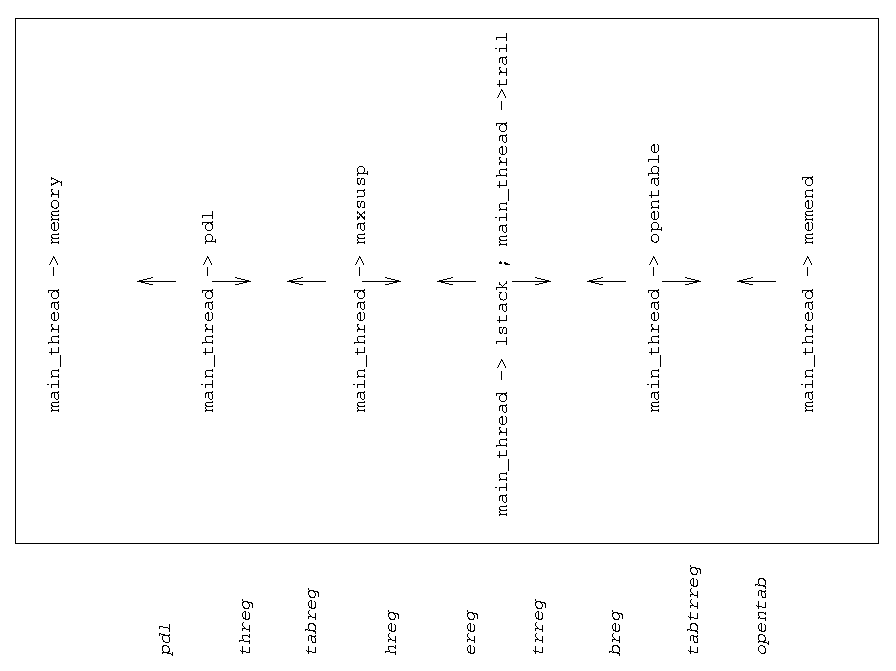
\psfig{file=figures/stack-layout.ps}}
\caption{Schematic Picture of XSB memory layout}\label{stack-layout.ps}
\end{figure}

Figure~\ref{tabspc.ps} shows the high-level structure of the table
space.  

\begin{figure}[htbp]
\mbox{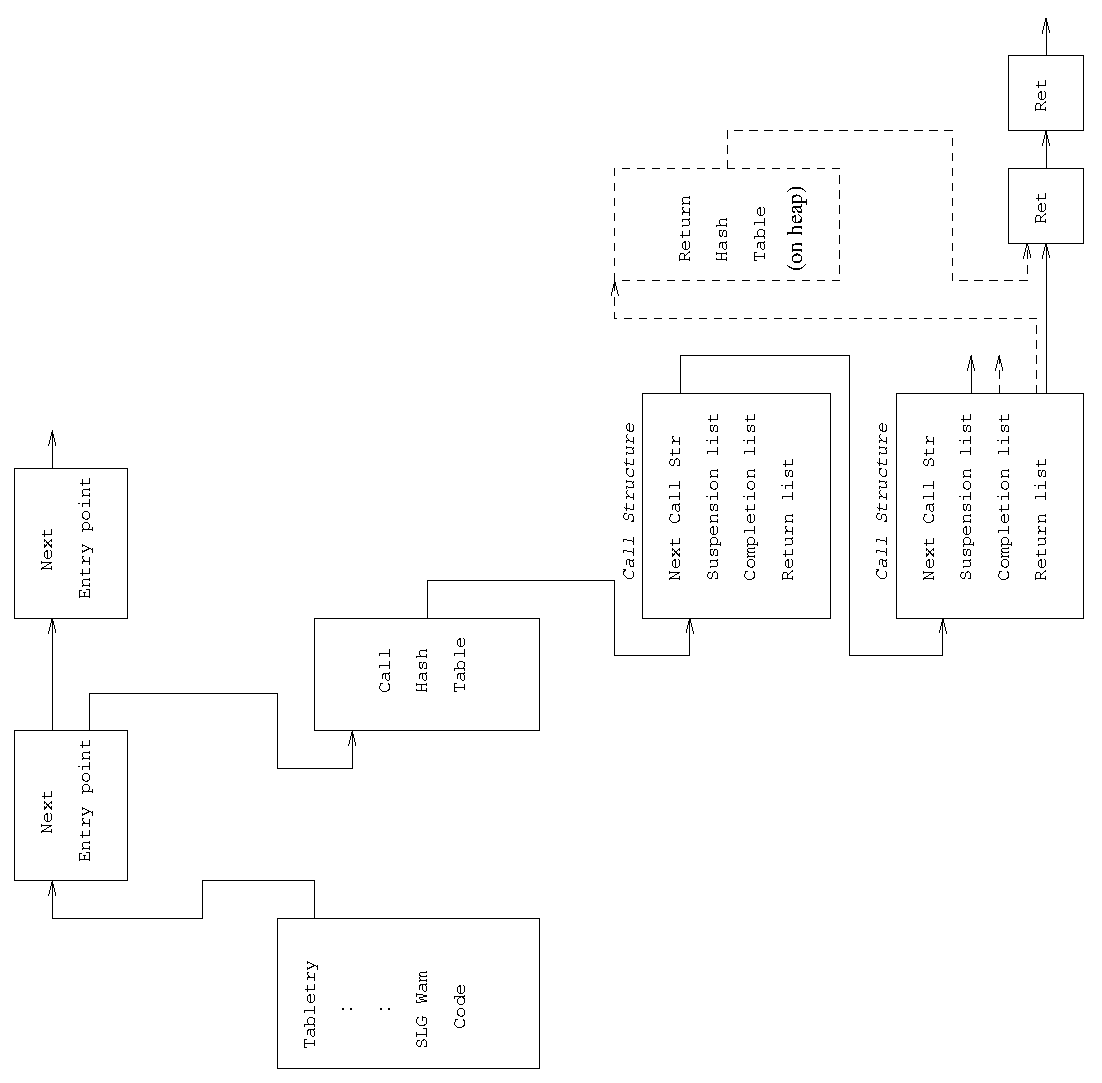
\psfig{file=figures/tabspc.ps}}
\caption{Schematic Picture of Table Space}\label{tabspc.ps}
\end{figure}

\begin{verbatim}
Table management Routines
	
	check_table_stack_overflow in choice.h
	saveinfo in xinst_fun copies from global.local into tablespace
	load_solution in xinst_fun copies into global.local from tablespace
	In addition to using table registers, they use the fact that
tables lie in virtual memory BELOW WAM stacks.  They will need to be
changed to make a check that tables are above WAM stacks.
	

Table Information Structures and pointers to them (tip)
	(grep on tip)

	-- typedef in xmacro.h, along with access macros.

	-- emu/psc.c contains a routine for finding a tip from a psc
pointer (pscs are explained in PSB tech ref manual).

	-- load_seg.c contains routines for initializing these
structures, using info from .O files.

	-- emu/builtin.c contains several builtins which access
information in tables through table information structures, and
'tip's, which are pointers to them.  The builtins are used mostly in
lib/tables.P.  (builtins generally are described in the PSB tech
reference manual).

Memory Management (such as it is) is in memory.h
	Space for program code is malloced as needed.
	Stack space is allocated once in init.c

Table abolishing routines.
	In tables.P

Debugging Routines
	In debug.c

hashindex.h
	This file culls out all call and return indexing routines, and
routines to traverse return lists.

\end{verbatim}

\subsection{Instruction-level Debugging}
%============================

The instruction level debugger is a powerful aid to improving the
emulator.  If you add or modify existing SLG-WAM instructions, you
will sooner or later need to use it or something like it.

Instruction level debugging can be involked from the interpreter in
two ways.  The most general way is to use the predicate {\tt
set\_pil\_on/0} from tables.P.  The goal
\begin{center} 
{\tt set\_pil\_on,p(X) }
\end{center}
will begin an instruction level trace with the call of {\tt p/1}.
Alternately adding the preprocessor directive
\begin{center}
\#define XTRACE
\end{center}
will begin an instruction level trace as soon as {\em xwammode} is
entered.  This condition holds from the time the first table in an
evaluation is entered until the time the last table is completed.

The debugger itself allows one to examine stacks and registers at each
instruction, to skip ahead a specified number of instructions, or to
set a memory or register watch to a particular value.  It is suggested
that debugging be done from a shell that allows scrolling and
searching, such as a shell invoked from emacs.

Each instruction is prinded out in the format
\begin{center}
{\em instruction-number instruction-address  instruction  parameters}
\end{center}
The instruction printed out will be executed {em next}.  After an
instruction or instructions are printed out, the debugger waits for a
prompt from the user.  Some useful values are presented below, but see
debug.c for a full set.  All addresses are assumed to be in
hexidecimal.

\begin{itemize}
	\item {\em q} quits 	
\item {\em d} dissasembles all loaded
code.  	
\item {\em r num} prints the cell value, and deref'ed value of
a register.  	
\item {\em R num} prints the cell value, and deref'ed
value of a register.  	
\item {\em v num} prints the value of a
permanent variable.  	
\item {\em a d num} prints the value at an
address.  	
\item {\em 1} prints table stack starting from tabreg.
Several lines are printed out and the user is prompted to continue.
\item {\em 2} prints table heap starting from threg.  Se
veral lines
are printed out and the user is prompted to continue.  
\item {\em P}
prints unification stack starting from pdlreg.  Several lines are
printed out and the user is prompted to continue.  	
\item {\em P}
prints unification stack starting from pdlreg.  Several lines are
printed out and the user is prompted to continue.  	
\item {\em p}
prints global stack starting from hreg.  Several lines are printed out
and the user is prompted to continue.  	
\item {\em e} prints local
stack starting from top of stack.  Several lines are printed out and
the user is prompted to continue.  	
\item {\em t} prints trail
starting from trreg.  Several lines are printed out and the user is
prompted to continue.  	
\item {\em c} prints choice point stack
starting from breg.  Several lines are printed out and the user is
prompted to continue.  
\item {\em C} prints choice point stack
starting from bfreg.  Several lines are printed out and the user is
prompted to continue.  	
\item {\em o} prints open table stack starting
from openreg.  Several lines are printed out and the user is prompted
to continue.  	
\item {\em S} prints values of registers.  	
\item {\em k num} skips {\em num} instructions, printing each instruction.
\item {\em K num} skips {\em num} instructions, without printing each
instruction. 
\item {\em w regnum num} sets register watch
\item {\em W stacknum num} sets memory watch
\end{itemize}

The register watch and memory watch bear further explanation.  The
register watch prints out a message whenever the register has a
particular value.  This is useful for determining when a program
might backtrack to a certain environment, say, or when a particular
binding is trailed.  The memory watch is similar, but prints out a
message whenever a particular address changes value, and is useful for
catching when bindings occurs.

There are also hooks from the instruction level debugger to the
interpreter level debugger, although these hooks can be shaky when
tabled code is traced, or when the dynamic loader is used.  See
debug.c for details.

When tracing tabling instructions, sets of printfs are spewn out when
the directives
\begin{center}
\#define XPIL
\#define XPIL1
\end{center}
or
\begin{center}
\#define OLDTTRACE
\end{center}
are written in main.c  XPIL dumps information about table
instructions, XPIL1 dumps information about indexing and table copy
subinstructions, and OLDTTRACE prints out information about table
calls and solutions.

\section                 {Miscellinious}
%                        ===============

\subsection{Save Status File Format}
%==================================

This subsection is to be rewritten due to the {\tt save} feature
is not tuned to the \version \mbox{} yet. The old format given below does
not work for the current version.

\begin{verbatim}
    4: 0x11121307        magic number

    4: pspace                start addr of pspace;
    4: maxspace                size of pspace;
    4: memory                start addr of local and heap stack
    4: maxmem                size of local and heap stack
    4: tstack                start addr of trail stack
    4: maxtrail                size of trail stack

    4: breg
    4: ereg
    4: hreg
    4: trreg
    4: hbreg
    4: cpreg
    4: pcreg

    4: nil_sym
    4: list_str
    4: list_psc
    4: comma_psc
    4: interrupt_psc
    8: trap_vector

    4: curr_fence        current top of pspace
    4: heap_used
    4: stack_used

    4: global_pair        ??? need to modify
    4: mod_list
    4: temp_list

    40: flags
    12: reg

subtotal: 160
pspace:   used portion
t-stack:  used portion
heap:     used portion
stack:    used portion
\end{verbatim}

\begin{thebibliography}{[8]}
 \bibitem[1]{sbprolog}
	Edited by Saumya Debray. {\it SB-Prolog Version 2.5 -- a user manual},
	September 1988.
\end{thebibliography}

\newpage

\appendix

\section		{Abstract Machine Instructions}
%			===============================

We list all abstract machine instructions below. All the instructions
are aligned with word (4 bytes) boundary with unused bytes padded.
This is necessary for running on machines with word alignment
restrictions such as Motorola 68000 (2 bytes alignment) or SPARC (4
bytes alignment). The size of instructions can be one, two or three
words. The opcode of the instruction takes the first byte in the first
(or the only) word, and the rest 3 bytes of the words are used for
arguments of one byte long. The second or the third word, if used,
always contain a single operand that requires the whole word.  

The
argument types listed in the table have the following meaning:

\begin{description}
  \item[A] one byte number for arity, size, built-in number, etc.
  \item[V] variable offset (one byte)
  \item[R] register number (one byte)
  \item[S] a structure (four bytes)
  \item[C] a constant (four bytes)
  \item[L] a label (address, four bytes)
  \item[G] a string
  \item[N] a number (integer or floating point, four bytes)
  \item[I] special; for the 2nd and 3rd arguments of switchonbound
  \item[P] pad, use a ``-'' in the table: the byte is not used (one byte)
  \item[PP] double pad, use two ``-'' in the table (two bytes)
  \item[PPP] triple pad, use three ``-'' in the table (three bytes)
\end{description}

\begin{tabbing}
Opcode\= Name Name Name \=Arg\=Arg\=Arg\= 2rd Word \= 3rd Word \= comments\kill
Opcode\> Name	\>A1 \>A2 \>A3 \>2rd Word\>3rd Word\>\hspace*{3em} Comments \\
\rule{\textwidth}{.01in}\\
0x00  \> getpvar	\> - \> V \> R \>   \>	 \>		\\
0x01  \> getpval	\> - \> V \> R \>   \>	 \>		\\
0x02  \> getstrv	\> - \> - \> V \> S \>   \>		\\
0x03  \> gettval	\> - \> R \> R \>   \>	 \>		\\
0x04  \> getcon		\> - \> - \> R \> C \>   \>		\\
0x05  \> getnil		\> - \> - \> R \>   \>   \>		\\
0x06  \> getstr		\> - \> - \> R \> S \>	 \>		\\
0x07  \> getlist	\> - \> - \> R \>   \>   \>		\\
0x08  \> unipvar	\> - \> - \> V \>   \>	 \>		\\
0x09  \> unipval	\> - \> - \> V \>   \>	 \>		\\
0x0a  \> unitvar	\> - \> - \> R \>   \>	 \>		\\
0x0b  \> unitval	\> - \> - \> R \>   \>	 \>		\\
0x0c  \> unicon		\> - \> - \> - \> C \>   \>		\\
0x0d  \> uninil		\> - \> - \> - \>   \>   \>		\\
0x0e  \> getnumcon	\> - \> - \> R \> N \>   \>		\\
0x0f  \> putnumcon	\> - \> - \> R \> N \>   \>		\\
0x10  \> putpvar	\> - \> V \> R \>   \>	 \>		\\
0x11  \> putpval	\> - \> V \> R \>   \>	 \>		\\
0x12  \> puttvar	\> - \> R \> R \>   \>	 \>		\\
0x13  \> putstrv	\> - \> - \> V \> S \>   \>		\\
0x14  \> putcon		\> - \> - \> R \> C \>   \>		\\
0x15  \> putnil		\> - \> - \> R \>   \>	 \>		\\
0x16  \> putstr		\> - \> - \> R \> S \>   \>		\\
0x17  \> putlist	\> - \> - \> R \>   \>	 \>		\\
0x18  \> bldpvar	\> - \> - \> V \>   \>   \>		\\
0x19  \> bldpval	\> - \> - \> V \>   \>   \>		\\
0x1a  \> bldtvar	\> - \> - \> R \>   \>	 \>		\\
0x1b  \> bldtval	\> - \> - \> R \>   \>	 \>		\\
0x1c  \> bldcon		\> - \> - \> - \> C \>   \>		\\
0x1d  \> bldnil		\> - \> - \> - \>   \>   \>		\\
0x1e  \> uninumcon	\> - \> - \> - \> N \>   \>		\\
0x1f  \> bldnumcon	\> - \> - \> - \> N \>   \>		\\
0x20  \>		\>   \>   \>   \>   \>	 \> not used	\\
---   \>		\>   \>   \>   \>   \>   \>		\\
0x47  \>		\>   \>   \>   \>   \>   \> not used	\\
0x48  \> getlist-tvar-tvar\>R\> R \> R \>   \>	 \>		\\
0x49  \> getcomma	\> - \> - \> R \>   \>   \> currently not used	\\
0x4a  \> getcomma-tvar-tvar\>R\>R \> R \>   \>   \> currently not used	\\
0x4b  \>		\>   \>   \>   \>   \>	 \> not used	\\
---   \>		\>   \>   \>   \>   \>   \>		\\
0x7f  \>		\>   \>   \>   \>   \>   \> not used	\\
0x80  \> getfloat	\> - \> - \> R \> N \>   \>		\\
0x81  \> putfloat	\> - \> - \> R \> N \>   \>		\\
0x82  \> unifloat	\> - \> - \> - \> N \>   \>		\\
0x83  \> bldfloat	\> - \> - \> - \> N \>   \>		\\
0x84  \>		\>   \>   \>   \>   \>	 \> not used	\\
---   \>		\>   \>   \>   \>   \>   \>		\\
0x99  \>		\>   \>   \>   \>   \>   \> not used	\\
0x9a  \> trys		\> - \> - \> A \> L \>   \>		\\
0x9b  \> retrys		\> - \> - \> A \> L \>   \>		\\
0x9c  \> trusts		\> - \> - \> A \> L \>   \>		\\
0x9d  \> neck		\> - \> - \> A \>   \>   \>		\\
0x9e  \> neck-putpbreg	\> - \> A \> V \>   \>	 \>		\\
0x9f  \> neck-puttbreg	\> - \> A \> R \>   \>	 \>		\\
0xa0  \> trymeelse	\> - \> - \> A \> L \>   \>		\\
0xa1  \> retrymeelse	\> - \> - \> A \> L \>   \>		\\
0xa2  \> trustmeelsefail\> - \> - \> A \>   \>   \>		\\
0xa3  \> try		\> - \> - \> A \> L \>   \>		\\
0xa4  \> retry		\> - \> - \> A \> L \>   \>		\\
0xa5  \> trust		\> - \> - \> A \> L \>   \>		\\
0xa6  \> getpbreg	\> - \> - \> V \>   \>   \>		\\
0xa7  \> gettbreg	\> - \> - \> R \>   \>	 \>		\\
0xa8  \> putpbreg	\> - \> - \> V \>   \>   \>		\\
0xa9  \> puttbreg	\> - \> - \> R \>   \>	 \>		\\
0xaa  \> jumptbreg	\> - \> - \> R \> L \>   \> used by dynamic preds\\
0xab  \> getarg-proceed \> - \> - \> A \>   \>   \> used by par-member	\\
0xac  \> getstring	\> - \> - \> R \> G \>   \>		\\
0xad  \> putstring	\> - \> - \> R \> G \>   \>		\\
0xae  \> unistring	\> - \> - \> - \> G \>   \>		\\
0xaf  \> bldstring	\> - \> - \> - \> G \>   \>		\\
0xb0  \> switchonterm	\> - \> - \> R \> L \> L \>		\\
0xb1  \> switchoncon	\> - \> - \> - \> L \>   \>		\\
0xb2  \> switchonstr	\> - \> - \> - \> L \>   \>		\\
0xb3  \> switchonbound	\> - \> - \> R \> I \> I \>		\\
0xb4  \>		\>   \>   \>   \>   \>	 \> not used	\\
0xb5  \>		\>   \>   \>   \>   \>   \> not used	\\
0xb6  \> suspend	\> - \> - \> - \>   \>   \> not used by compiler \\
0xb7  \> partry		\> - \> - \> A \> N \>   \>		\\
0xb8  \> terminate	\> - \> - \> - \>   \>   \> not used by compiler \\
0xb9  \>		\>   \>   \>   \>   \>	 \> not used	\\
---   \>		\>   \>   \>   \>   \>   \>		\\
0xd0  \>		\>   \>   \>   \>   \>   \> not used	\\
0xd1  \> movreg		\> - \> R \> R \>   \>	 \>		\\
0xd2  \> negate		\> - \> - \> R \>   \>	 \>		\\
0xd3  \> and		\> - \> R \> R \>   \>	 \>		\\
0xd4  \> or		\> - \> R \> R \>   \>	 \>		\\
0xd5  \> logshiftl	\> - \> R \> R \>   \>	 \>		\\
0xd6  \> logshiftr	\> - \> R \> R \>   \>	 \>		\\
0xd7  \> addreg		\> - \> R \> R \>   \>	 \>		\\
0xd9  \> subreg		\> - \> R \> R \>   \>	 \>		\\
0xd9  \> mulreg		\> - \> R \> R \>   \>	 \>		\\
0xda  \> divreg		\> - \> R \> R \>   \>	 \>		\\
0xdb  \> idivreg	\> - \> R \> R \>   \>	 \>		\\
0xdc  \>		\>   \>   \>   \>   \>	 \> not used	\\
---   \>		\>   \>   \>   \>   \>   \>		\\
0xdf  \>		\>   \>   \>   \>   \>   \> not used	\\
0xe0  \> putdval	\> - \> V \> R \>   \>	 \>		\\
0xe1  \> putuval	\> - \> V \> R \>   \>	 \>		\\
0xe2  \> getival	\> - \> - \> A \> S \>   \> not used by compiler \\
0xe3  \>		\>   \>   \>   \>   \>	 \> not used	\\
---   \>		\>   \>   \>   \>   \>   \>		\\
0xe6  \>		\>   \>   \>   \>   \>   \> not used	\\
0xe7  \> unexec		\> - \> - \> - \> S \> S \> not used by compiler \\
0xe8  \> call		\> - \> - \> A \> S \>   \>		\\
0xe9  \> allocate	\> - \> - \> - \>   \>   \>		\\
0xea  \> deallocate	\> - \> - \> - \>   \>   \>		\\
0xeb  \> proceed	\> - \> - \> - \>   \>   \>		\\
0xec  \> execute	\> - \> - \> - \> S \>   \>		\\
0xed  \> unexeci	\> - \> - \> - \> S \> S \> not used by compiler \\
0xee  \> executev	\> - \> - \> - \> S \>   \>		\\
0xef  \> calld		\> - \> - \> A \> L \>   \>		\\
0xf0  \> jump		\> - \> - \> - \> L \>   \>		\\
0xf1  \> jumpz		\> - \> - \> R \> L \>   \>		\\
0xf2  \> jumpnz		\> - \> - \> R \> L \>   \>		\\
0xf3  \> jumplt		\> - \> - \> R \> L \>   \>		\\
0xf4  \> jumple		\> - \> - \> R \> L \>   \>		\\
0xf5  \> jumpgt		\> - \> - \> R \> L \>   \>		\\
0xf6  \> jumpge		\> - \> - \> R \> L \>   \>		\\
0xf7  \> cases		\> A \> N \> N \>   \>   \> 
					10 bytes; not used in emulator \\
0xf8  \> fail		\> - \> - \> - \>   \>   \>		\\
0xf9  \> noop		\> - \> - \> A \>   \>   \>		\\
0xfa  \> halt		\> - \> - \> - \>   \>   \>		\\
0xfb  \> builtin	\> - \> - \> A \>   \>   \>		\\
0xfc  \> unifunc	\> - \> A \> R \>   \>	 \>		\\
0xfd  \> userfunc	\> - \> - \> R \> S \>   \>		\\
0xfe  \> 		\>   \>   \>   \>   \>   \> not used	\\
0xff  \> endfile	\> - \> - \> - \> N \>   \> not used any more	\\
0000  \> label		\> T \> L \>   \>   \>   \> used only in assembler \\
0000  \> arglabel	\> T \> I \> L \>   \>   \> used only in assembler \\
0000  \> modname	\>   \>   \>   \>   \>   \> used only in assembler \\
\end{tabbing}



\section		{Primitive Predicates}
%			======================


\begin{tabbing}
Number \= 1234567890123456789012345678901234567890 \= Comment \kill
Number	\> Name				\> 	Comment		\\
------ \> ------------------------------\>------------------------\\
 1 \> psc\_name(PSC, String)		\>			\\
 2 \> psc\_arity(PSC, Arity)		\>			\\
 3 \> psc\_type(PSC, Type)		\>			\\
 4 \> psc\_prop(PSC, Term)		\>			\\
 5 \> psc\_set\_type(PSC, Type, Perm)	\>			\\
 6 \> psc\_set\_prop(PSC, Term, Perm)	\>			\\
 7 \> file\_open(NameString, RWMode, File)\>			\\
 8 \> file\_close(File)			\>			\\
 9 \> file\_get(File, Char)		\>			\\
10 \> file\_put(File, Char)		\>			\\
11 \> term\_psc(Term, PSC)		\>			\\
12 \> term\_type(Term, Type)		\>			\\
13 \> term\_compare(Term1, Term2, Res)	\>			\\
14 \> term\_new(PSC, Term)		\>			\\
15 \> term\_arg(Term, Index, Arg)	\>			\\
16 \> term\_set\_arg(Term, Index, Arg, Perm)\>			\\
17 \> stat\_flag(Flag, Value)		\>			\\
18 \> stat\_set\_flag(Flag, Value, Perm)\>			\\
19 \> buff\_alloc(Size, Buffer, Perm)	\>			\\
20 \> buff\_word(Buffer, Disp, Value)	\>			\\
21 \> buff\_set\_word(Buffer, Disp, Value)\>			\\
22 \> buff\_byte(Buffer, Disp, Value)	\>			\\
23 \> buff\_set\_byte(Buffer, Disp, Value)\>			\\
24 \> code\_call(CodeAddr, Term, Type)	\>			\\
25 \> str\_len(String, Length)		\>			\\
26 \> str\_cpy(String1, Buffer)		\>			\\
27 \> str\_cat(String1, String2, String3)\>			\\
28 \> str\_cmp(String1, String2, Res)	\>			\\
29 \> str\_hsh(String, Arity, Size, Res)\>			\\
30 \> str\_insert(InString, OutString)	\>			\\
32 \> stat\_sta(X)			\>			\\
33 \> stat\_cputime(X)			\>			\\
34 \> code\_load(ByteCodeFileName, InitAddr)\>			\\
35 \> buff\_set\_var(Buffer, Disp, BufferSize, Var)\>		\\
36 \> buff\_dealloc(Buffer, OldSize, NewSize, Perm)\>		\\
37 \> buff\_cell(Buffer, Disp, Term)	\>			\\
38 \> buff\_set\_cell(Buffer, Disp, Type, Value)\>		\\
40 \> file\_getword(File, Word)		\>			\\
41 \> file\_putword(File, Word)		\>			\\
42 \> psc\_insert(Name, Arity, PSC, MName)\>			\\
43 \> psc\_import(Pname, Arity, Mname)	\>			\\
44 \> file\_getbuf(File, Bytes, Buf, Disp)\>			\\
45 \> file\_putbuf(File, Bytes, Buf, Disp)\>			\\
46 \> psc\_insertmod(ModName, Def, PSC)	\>			\\
47 \> load\_seg(SegNo, TextBytes, IndexBytes, File, InitAddr)\>		\\
48 \> file\_gettoken(File, Char, Type,	Value, NextChar)\>		\\
49 \> file\_puttoken(File, Type, Value)	\>			\\
50 \> term\_hash(Term,TableSize,Value)	\>			\\
51 \> unload\_seg(Addr)			\>			\\
52 \> load\_obj(OFile,Mod,LdOption,InitAddr) \>			\\
55 \> sys\_syscall(CallNo,Res,Arg,\ldots) \>			\\
56 \> sys\_system(Command, Result)	\>			\\
57 \> sys\_gethost(Name, Buffer)	\>			\\
58 \> sys\_errno(Errno)			\>			\\
59 \> sys\_brocall(CallNo,Arg,Res)	\>			\\
60 \> lock\_destroy(Lock)		\>			\\
61 \> lock\_init(Lock)			\>			\\
62 \> lock\_on(Lock)			\>			\\
63 \> lock\_off(Lock)			\>			\\
80 \> dom\_size(Dom, Size)		\>			\\
81 \> dom\_type(Dom, Type)		\>			\\
82 \> dom\_range(Dom, Min, Max)		\>			\\
83 \> dom\_elem(Dom, Index)		\>			\\
84 \> dom\_diff(X, Y, Z)		\>			\\
85 \> dom\_plus(X, Y, Z)		\>			\\
86 \> dom\_times(X, Y, Z)		\>			\\
87 \> dom\_min(Dom, Min)		\>			\\
88 \> dom\_enum(Dom, TypePsc)		\>			\\
89 \> dom\_esize(Dom, Size)		\>			\\
96 \> buff\_assign\_word(Buff,Disp,Value) \>			\\
97 \> par\_member\_try(X, Term, Size)	\>			\\
\end{tabbing}

\section		{Emulator Flags}
%
\label{s:emuflags}

The set of emulator flags are listed below.

\begin{center}
\begin{tabular}{l|l|l}
\hline
C variable name & Number & Comment				\\
\hline
pil\_trace	&  0        & for system debugger		\\
hitrace		&  1        & for system debugger		\\
overflow\_f     &  2        & when 1, ignore stack overflow	\\
trace\_sta      &  3        & record statistics			\\
debug\_on       &  4        & debugging mode on			\\
hide\_state     &  5        & hide debugging			\\
trace           &  6        & trace mode on			\\
invoke\_num     &  7        & invoking number, for debugger	\\
skipping        &  8        & skipping during debugging		\\
quasi\_skipping &  9        & quasi-skipping during debugging	\\
current\_input  & 10        & current input stream		\\
current\_output & 11        & current output stream		\\
current\_module & 12        & current module (pointer to the module symbol) \\
mod\_list       & 13        & the module symbol list		\\
reloc\_table    & 14        & relocation table, can only ``get''\\
hash\_table	& 15	    & hash table address; can only ``get'' \\
version\_major	& 16	    & major version number; get only	\\
version\_minor	& 17	    & minor version number; get only	\\
version\_word	& 18	    & word format (get only); 1 - SW, 2 - HW, 3 - DW \\
version\_mode	& 19	    & emulator mode (get); 1 - optimal, 2 - debug, 
					3 - profile \\
version\_para	& 20	    & parallel mode (get); 1 - sequential,  
					2 - parallel \\
version\_procr	& 21	    & number of processors		\\
version\_date	& 22	    & the date of the emulator creation \\
install\_dir	& 23	    & the directory that the system resides \\
get\_worker	& 24	    & not used any more			\\
woken\_delay	& 25	    & list of woken delayed goals \\
delay\_head\_ptr& 26	    & delayed goal list \\
hostmachine	& 27	    & 1 - Sun; 2 - sequent		\\
pil\_step	& 28	    & for system debugger		\\
call\_step	& 29	    & for system debugger		\\
thread\_step	& 30	    & for system debugger		\\
showthread	& 31	    & for system debugger		\\
flags[32--47]	& 32--47    & interrupt vectors			\\
USER\_HOME	& 49	    & User's home directory		\\
LIBS\_LOADED	& 50	    & 0=default libpath, 1=user+def libpath \\
XTRACEFLAG      & 51	    & xwam level tracing is on		\\
PROFFLAG        & 52	    & profiling is on			\\
flags[53--63]	& 48--63    & user defined flags \\
\hline
\end{tabular}
\end{center}


\end{document}
